\section{DK-5300 PC Software}
\label{cha:DK5300}

\subsection{General Information}
DK-5300 is a Windows\registeredtm program that enables you to configure and remote control PT5300's connected to your LAN (Local Area Network).\\
The latest version of DK-5300.EXE can always be found on our web site \href{http://www.dk-technologies.com}{www.dk-technologies.com}.\\

\begin{figure}[hbt]
\centering
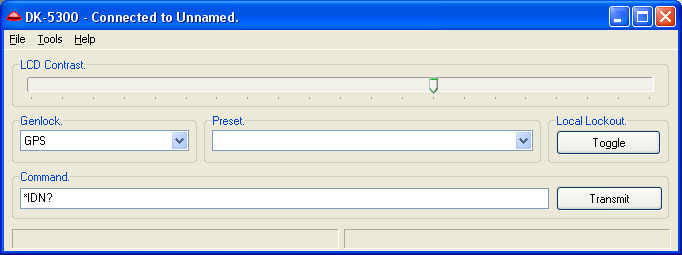
\includegraphics[width=1\textwidth]{fig/DK5300_MainWindow}
\caption{The DK-5300 main window.\label{fig:DK5300MainWindow}}
\end{figure}

The configuration of the PT5300 network settings are done using the NetFinder protocol. This enables you to configure the IP address, User name, Password, etc... on multiple PT5300's from one single location. The network port for the NetFinder protocol is 3040 (UDP).

The normal remote commands described in section \ref{cha:Remote} are transmitted using the Telnet protocol. The default port for Telnet is 23 (TCP).\\
\PasswordWarning
\newpage
\subsection{Connect to the PT5300.}
\label{cha:DK5300Connect}
\textbf{Operation:}

\begin{itemize}
\item Start the DK-5300.EXE and allow the program to connect to the network.
	\begin{itemize}
		\item The NetFinder protocol uses port 3040.
		\item The Telnet port can be changed but as default Telnet uses port 23.
	\end{itemize}
\item When the main window of DK-5300 is visible, go to the menu ``File'' and select ``NetFinder''.
\item When the NetFinder window is visible, click ``Refresh Instrument List''.

\begin{figure}[hbt]
\centering
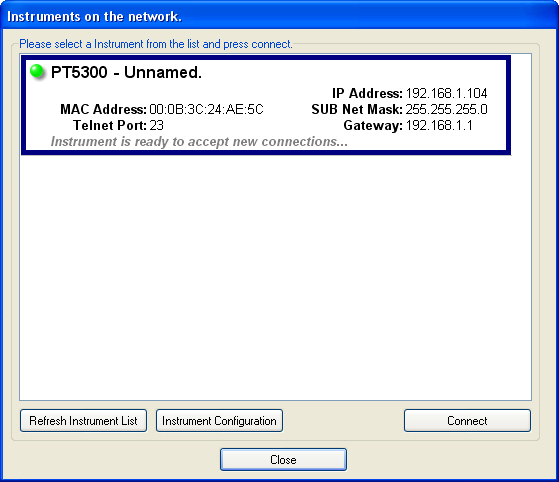
\includegraphics[width=0.6\textwidth]{fig/NetFinder_Search}
\caption{The NetFinder Window.\label{fig:NetFinderWindow}}
\end{figure}

	\begin{itemize}
		\item DK-5300 will now search the LAN for PT5300's. This process takes 10 seconds.
		\item During the search, PT5300's will be added to the list in the NetFinder window. Instruments are added in the order they are discovered.
		\item It is possible to connect to a PT5300 while the search is in progress.
%		\item From the NetFinder window it is also possible to change network settings for a PT5300.
		\item Each item in the instrument list will show the instrument type, the user configurable NetFinder name, the connection status of the instrument and optionally the IP settings of the instrument and Telnet port.\\\\
		\textbf{Connection status.}\\
					\raisebox{-0.5ex}{
\includegraphics{fig/Bubble_Green_Shadow}} - The Instrument is ready to accept new connections.\\
					\raisebox{-0.5ex}{
\includegraphics{fig/Bubble_Yellow_Shadow}} - The Instrument is busy. A connection has been established from another computer.\\
					\raisebox{-0.5ex}{
\includegraphics{fig/Bubble_Red_Shadow}} - Login in progress. A connection is being established from another computer.\\
					\raisebox{-0.5ex}{
\includegraphics{fig/Bubble_Grey_Shadow}} - Instrument is unavailable. The Telnet protocol has been disabled locally on the PT5300.\\
					\textit{	Please see section \ref{cha:NETWORK} for information about how to enable or disable the Telnet protocol.}
	\end{itemize}
\item Select from the instrument list the PT5300 you wish to connect to and press ``Connect''.
	\begin{itemize}
		\item You will be asked for the user name and password.
		\item The default user name is \textbf{\DefaultUser}. (Case sensitive.)
		\item The default password is \textbf{\DefaultPass}. (Case sensitive.)
		\item If ``Remember Login'' is checked the user name and password is saved in the DK-5300 configuration file.

		\begin{figure}[hbt]
		\centering
		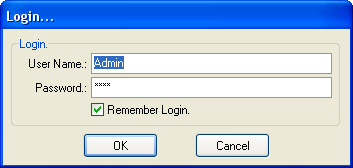
\includegraphics[width=0.3\textwidth]{fig/Login}
		\caption{The Login dialog.\label{fig:LoginDialog}}
		\end{figure}

	\end{itemize}
\item When a connection with a PT5300 has been established, the main window will then show basic options for remote control. \textit{(Figure \ref{fig:DK5300MainWindow}).}
	\begin{itemize}
		\item \textbf{LCD Contrast:} Set the LCD contrast.
		\item \textbf{Genlock:} Select the genlock source.
		\item \textbf{Preset:} Select the active preset. The dropdown box will show the active preset. If no preset is active the dropdown box will be empty.
		\item \textbf{Local Lockout:} Toggle whether or not the PT5300 responds to the local user interface.
		\item \textbf{Command:} Enter a command and press ``Transmit'' to send a specific command to the PT5300. Please see section \ref{cha:CommandRef} for further information about valid commands. There will be no indication whether or not the command has been executed unless the command is a query command.
	\end{itemize}
\end{itemize}

\subsection{Change network configuration.}
\label{cha:DK5300Configuration}

\textbf{Operation:}

\begin{itemize}
\item Open the NetFinder window.
	\begin{itemize}
		\item From the main window select ``File'' -> ``NetFinder''.
	\end{itemize}
\item When the NetFinder window is visible, click ``Refresh Instrument List''. \textit{(Figure \ref{fig:NetFinderWindow}).}
\item Select from the instrument list the PT5300 you wish to configure and press ``Instrument Configuration''.
\item The Instrument Configuration window will appear.

\begin{figure}[hbt]
\centering
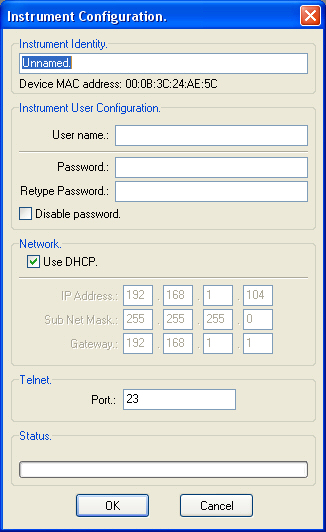
\includegraphics[width=0.28\textwidth]{fig/NetFinder_Config}
\caption{The Instrument Configuration Window.\label{fig:NetFinderConfigWindow}}
\end{figure}
\item	\textbf{Configuration options.}\\
	\begin{itemize}
		\item \textbf{Instrument Identity:}\\The text field allows you to change the NetFinder name. When multiple PT5300's are connected to the LAN the NetFinder name is used for easy identification in the Instrument List \textit{(Figure: \ref{fig:NetFinderWindow})}.\\The NetFinder name is also shown in the main window of DK-5300 when a connection with the instrument has been established.
		\item \textbf{Instrument User Configuration:}\\The text field ``User Name'' allows you to change the default user name. If this field is left blank no changes will be made to the user name.\\The password fields allows you to change the default password. The two password fields must match each other. The password can be disabled by checking ``Disable Password''. If the password fields are left blank, no changes will be made to the password.
		\item \textbf{Network.}\\The instrument is by default configured to use DHCP. This can be disabled by un-checking DHCP. When DHCP is disabled the text fields for IP configuration is enabled. If you enter the wrong IP settings you might not be able to reconnect to the instrument.\\\\\textbf{The DHCP and IP settings can always be reconfigured locally on the instrument. Please see section \ref{cha:NETWORK} for further information about how to do this.}
		\item \textbf{Telnet:}\\The default Telnet port is 23. In the Telnet field this can be changed. The Telnet port can be configured to a value between 1 and 65535.
	\end{itemize}
\item Click ``OK'' to apply the changes. If ``Cancel'' is selected the changes will be discarded.
	\begin{itemize}
		\item When you apply the changes you will be asked for the user name and password. \textit{(Figure \ref{fig:LoginDialog}).}
		\item The default user name is \textbf{\DefaultUser}. (Case sensitive.)
		\item The default password is \textbf{\DefaultPass}. (Case sensitive.)
		\item If ``Remember Login'' is checked the user name and password is saved in the DK-5300 configuration file.
		\item A message box will then appear stating whether or not the changes have been accepted by the instrument.
		\item When the configuration has been changed you should wait approximately 30 seconds for the changes to take effect and then refresh the instrument list.
	\end{itemize}
\end{itemize}
The instrument can not be reconfigured using the NetFinder protocol while a Telnet connection is active.\\If the network settings are changed locally on the instrument (please see section \ref{cha:NETWORK} for further information) all connections will be disconnected while reloading the new configuration.
\newpage
\subsection{DK-5300 Options}
\textbf{Operation:}

\begin{itemize}
\item Open the option window.
	\begin{itemize}
		\item From the main window select ``Tools'' -> ``Options...''.
	\end{itemize}
\item The option window currently have two options.

\begin{figure}[hbt]
\centering
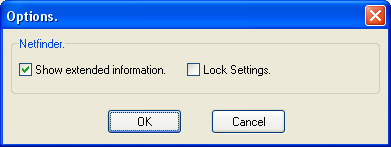
\includegraphics[width=0.35\textwidth]{fig/DK5300_Options}
\caption{The DK-5300 Option Window.\label{fig:DK5300OptionWindow}}
\end{figure}
	\begin{itemize}
		\item \textbf{Show extended information:}\\When checked, the instrument list in the NetFinder window will show the MAC address, Telnet Port and IP information for every instrument discovered on the LAN. If un-checked, only the NetFinder name and connection status is shown. \textit{(Figure: \ref{fig:NetFinderWindow})}
		\item \textbf{Lock Settings:}\\When checked, the ``Instrument Configuration'' function in the NetFinder window will be disabled.
	\end{itemize}
\item Click ``OK'' to apply the changes. If ``Cancel'' is selected the changes will be discarded.
\end{itemize}

\clearpage
